\documentclass[a4paper, 14pt]{extarticle}

\usepackage{../latexDependencies/misc/preamble2}

\geometry{a4paper}

% Название дисциплины
\newcommand{\subject}{Теория вероятности и математическая статистика} 

% Тип работы
% lab - для лабораторной работы 
% hw  - для домашней     работы
\newcommand{\task}{lab} 

% Номер работы
\newcommand{\taskNumber}{4} 

% Название работы
\newcommand{\taskNameOne}{Интервальные оценки для параметра } 
\newcommand{\taskNameTwo}{биноминального закона.} 

% Имя студента
\newcommand{\studentName}{Очкин Н.В.}

% Имя преподававателя
\newcommand{\teacherName}{Облакова Т.В.}

% Группа
\newcommand{\group}{ФН11-52Б}

% Вариант
\newcommand{\variant}{9}

\begin{document}

\graphicspath{ {../latexDependencies/images} } 
\normalsize

\newcommand{\printTask}{%
    \ifthenelse{\equal{\task}{lab}}{%
        лабораторной%
    }{%
        \ifthenelse{\equal{\task}{hw}}{%
            домашней%
        }{%
            Неизвестный тип задания%
        }%
    }%
}

\begin{titlepage}

    \begin{center}
        {\footnotesize \itshape Федеральное государственное бюджетное 
                       образовательное учреждение высшего образования}
    \end{center}

    \begin{minipage}[c]{0.1\textwidth}
        
\includegraphics[width=1.1\textwidth]{iconBMSTU}
    \end{minipage}
    \hfill
    \begin{minipage}[c]{0.9\textwidth}
        \centering
        \itshape
        \bfseries
        \small
        \guillemotleft Московский государственный технический университет \\
        имени Н.Э. Баумана\guillemotright \\
        (национальный исследовательский университет) \\
        (МГТУ им. Н.Э. Баумана) 
    \end{minipage}

    \vspace{0.5cm}
    \noindent\rule{\textwidth}{2pt} \\

    \noindent\uline{\textbf{ФАКУЛЬТЕТ} ФУНДАМЕНТАЛЬНЫЕ НАУКИ} \\
    \vspace{-5pt} \\
    \noindent\uline{\textbf{КАФЕДРА} ВЫЧИСЛИТЕЛЬНАЯ МАТЕМАТИКА И МАТЕМАТИЧЕСКАЯ} \\
    \vspace{-5pt} \\
    \noindent\uline{ФИЗИКА (ФН11)} \\
    \vspace{-5pt} \\
    \noindent\uline{\textbf{НАПРАВЛЕНИЕ ПОДГОТОВКИ} МАТЕМАТИКА И КОМПЬЮТЕРНЫЕ} \\
    \vspace{-5pt} \\
    \noindent\uline{НАУКИ (02.03.01)} \\

    \begin{center}
        \bfseries
        \textsc{О т ч е т} \\[10pt]
        по \printTask {} работе \textnumero {} \taskNumber
    \end{center}

    \vspace{10pt}

    \hspace{10pt} 
    \noindent \textbf{Название \printTask {} работы:} \par
    \vspace{5pt}
    \hspace{10pt} 
    \noindent \textbf{\uline{\taskNameOne}} \vspace{5pt} \\
    \null\hspace{31pt} 
    \textbf{\uline{\taskNameTwo}} \vspace{5pt} 

    \vspace{10pt}

    \begin{center}
        \bfseries
        Вариант \textnumero {} \variant
    \end{center}

    \vspace{20pt}

    \hspace{10pt} 
    \noindent \textbf{Дисциплина:} \par
    \vspace{10pt}
    \hspace{10pt} 
    \noindent {\large \subject}

    \vspace{10pt}

    \begin{flushright}
        \renewcommand{\arraystretch}{3}
        \begin{tabular}{r r r}
            \multicolumn{1}{l}{Студент группы \uline{\group}} & 
            $\quad \underset{\text{(Подпись, дата)}}{\underline{\hspace{3cm}}} \quad$ & 
            \multicolumn{1}{c}{$\underset{\text{(И.О. Фамилия)}}{\uline{\textbf{\studentName}}}$} \\

            \multicolumn{1}{l}{Преподаватель} & 
            $\quad \underset{\text{(Подпись, дата)}}{\underline{\hspace{3cm}}} \quad$ & 
            \multicolumn{1}{c}{$\underset{\text{(И.О. Фамилия)}}{\uline{\textbf{\teacherName}}}$} \\
        \end{tabular}
    \end{flushright}

    \vfill

    \begin{center}
        \small
        Москва, 2024
    \end{center}
\end{titlepage}


\newgeometry{left=25mm, right=25mm, top=20mm, bottom=20mm}

\graphicspath{ {../latexDependencies/images/LW4} }

% Customize section, subsection, subsubsection and paragraph styles
\titleformat{\section}
  {\normalfont\large\bfseries}{\thesection}{1em}{}

\titleformat{\subsection}
  {\normalfont\normalsize\bfseries}{\thesubsection}{1em}{}

\titleformat{\subsubsection}
  {\normalfont\small\bfseries}{\thesubsubsection}{1em}{}

\titleformat{\paragraph}
  {\small\small\bfseries}{\theparagraph}{1em}{}

\thispagestyle{empty}

\null\newpage

% \setcounter{tocdepth}{5}
% \setcounter{secnumdepth}{5}

% \pagenumbering{roman}

% \tableofcontents
% \newpage

\pagenumbering{arabic}
\setcounter{page}{1}

\setstretch{1}
\linespread{1.1}

\setlength{\parindent}{0pt}

\fontsize{12pt}{16pt}\selectfont

\definecolor{myblue}{HTML}{0A88C2}
\definecolor{myred}{HTML}{FF1B1C}
\definecolor{mygreen}{HTML}{386641}

\lstdefinestyle{mystyle}{
    basicstyle=\ttfamily\footnotesize,
    keywordstyle=\color{myblue},
    stringstyle=\color{myred},
    commentstyle=\color{green!50!black},
    showstringspaces=false,
    frame=leftline, 
    framesep=10pt, 
}

% Set the style for Python code
\lstset{style=mystyle, extendedchars=\true}

% --------------------------------------START--------------------------------------

\section*{Задание}\vspace{-20pt}\rule{\linewidth}{0.1mm}

\begin{enumerate}
    \item Используя выборку, сгенерированную вами в задаче 2 и считая параметр $p$ неизвестным ($k$-дано), постройте для уровней доверия 1-$\alpha$=0.9, 0.95 и 0.98 симметричные интервальные оценки Клоппера-Пирсона ( $\underline{p}$; $\overline{p}$) для вероятности успеха в одном испытании $p$.
    \item Для тех же уровней найдите по ЦПТ приближенные доверительные интервалы для $p$.
    \item Сравните полученные результаты и убедитесь, что полученные интервалы содержат истинное значение параметра.
    \item Для одного из значений $\alpha$ постройте совмещенные графики функций распределения биномиальных законов $B(k,p)$, $B(k,\underline{p})$, $B(k,\overline{p})$.
    \item Сформулируйте выводы.
\end{enumerate}

\section*{Исходные данные}\vspace{-20pt}\rule{\linewidth}{0.1mm}

\begin{equation*}
    k = 8 \qquad p = 0.7 \quad n = 140 \quad \alpha = 0.1,\quad 0.05,\quad 0.02,\quad 0.01
\end{equation*}

\begin{table}[h!]
    \centering
    \begin{tabular}{|>{\centering\arraybackslash}p{0.5cm}|>{\centering\arraybackslash}p{0.5cm}|>{\centering\arraybackslash}p{0.5cm}|>{\centering\arraybackslash}p{0.5cm}|>{\centering\arraybackslash}p{0.5cm}|>{\centering\arraybackslash}p{0.5cm}|>{\centering\arraybackslash}p{0.5cm}|>{\centering\arraybackslash}p{0.5cm}|}
    \hline
    7 & 6 & 5 & 8 & 4 & 3 & 6 & 7 \\ \hline
    5 & 6 & 4 & 7 & 7 & 6 & 5 & 6 \\ \hline
    6 & 6 & 2 & 6 & 6 & 5 & 5 & 7 \\ \hline
    7 & 6 & 7 & 6 & 7 & 7 & 5 & 4 \\ \hline
    2 & 5 & 5 & 8 & 6 & 5 & 7 & 6 \\ \hline
    4 & 6 & 3 & 5 & 6 & 1 & 8 & 6 \\ \hline
    7 & 6 & 7 & 5 & 8 & 6 & 5 & 7 \\ \hline
    5 & 4 & 6 & 8 & 7 & 4 & 5 & 7 \\ \hline
    6 & 6 & 5 & 5 & 6 & 7 & 6 & 7 \\ \hline
    5 & 7 & 5 & 6 & 7 & 5 & 6 & 5 \\ \hline
    5 & 7 & 6 & 5 & 5 & 4 & 5 & 7 \\ \hline
    6 & 3 & 4 & 6 & 5 & 4 & 6 & 7 \\ \hline
    7 & 4 & 6 & 3 & 7 & 5 & 5 & 6 \\ \hline
    7 & 4 & 7 & 5 & 5 & 6 & 4 & 6 \\ \hline
    7 & 6 & 3 & 5 & 6 & 6 & 5 & 7 \\ \hline
    6 & 4 & 5 & 7 & 6 & 7 & 5 & 6 \\ \hline
    6 & 4 & 3 & 7 & 4 & 4 & 4 & 5 \\ \hline
    7 & 8 & 5 & 5 & 7 & 5 &   &   \\ \hline
    \end{tabular}
\end{table}

\section*{Выполнение работы}\vspace{-20pt}\rule{\linewidth}{0.1mm}

По условию, параметр $p$ подразумеваем неизвестным, в то время  как  значение 
$k$ = 8 считаем  данным. В результате моделирования были получены значения выборочного 
среднего $\overline{X}$ и статистики $K(\overrightarrow{X}_n)$.

\begin{center}
    \begin{lstlisting}[language=Python]
overlineX = 1 / len(X) * sum(X)

K_Stat = sum(X)
    \end{lstlisting}
\end{center}

\vspace{-10pt}

\begin{equation*}
    \overline{X} = 5.593 \qquad K(\overrightarrow{X}_n) = 783
\end{equation*}

Приведем графики квантилей для $\alpha = 0.01$ в зависимости от $p$ и отметим значение 
$K(\overrightarrow{X}_n)$.

\begin{center}
    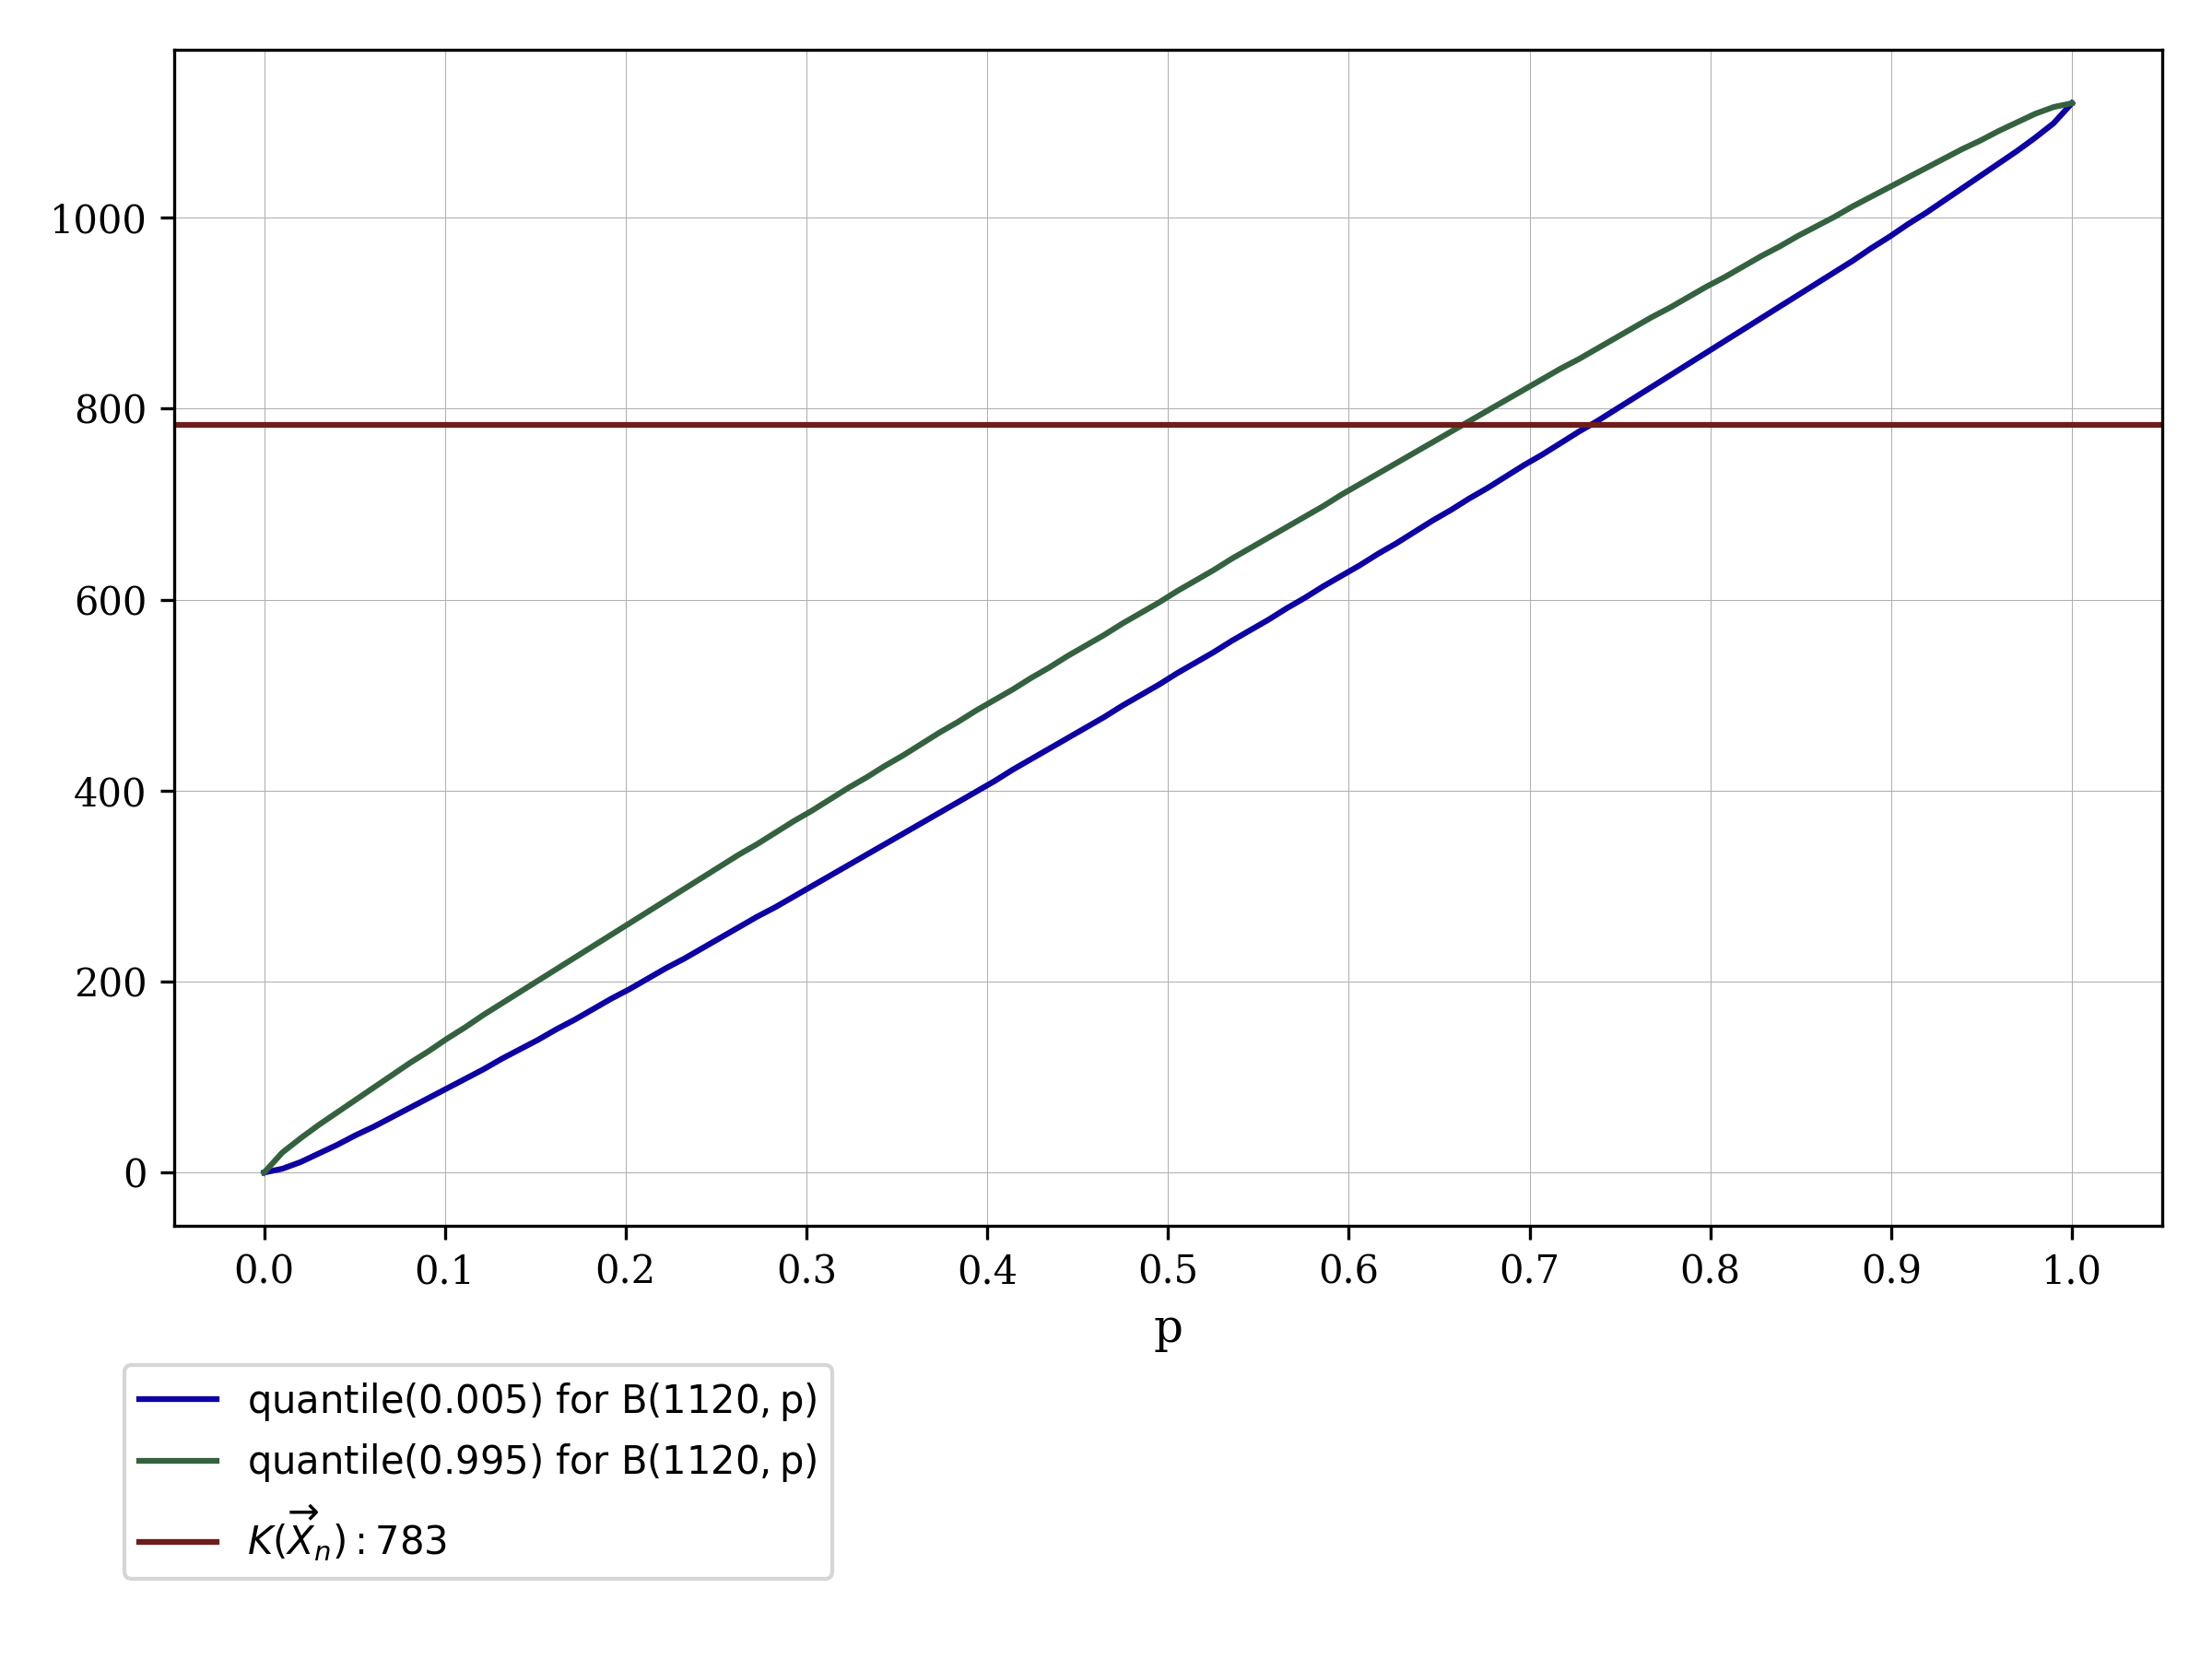
\includegraphics[width=1\textwidth]{quantiles}
\end{center}

Численно найдем точки пересечения для различных значений $\alpha$. Таким образом найдем 
приближенные значения $\underline{p}$ и $\overline{p}$.

\begin{center}
    \begin{lstlisting}[language=Python]
alphas_ = [0.1, 0.05, 0.02, 0.01]

quantile = lambda alpha, n, p : sp.stats.binom.ppf(alpha, n, p)

for alpha in alphas_:

    foo1 = lambda p : quantile(1 - alpha / 2, n_*k_, p) - K_Stat
    foo2 = lambda p : quantile(alpha/2, n_*k_, p) - K_Stat

    underlineP = sp.optimize.brentq(foo1, 0, 1, xtol=1e-6)
    overlineP  = sp.optimize.brentq(foo2, 0, 1, xtol=1e-6)
    \end{lstlisting}
\end{center}

\vspace{-10pt}

\begin{alignat*}{3}
    \alpha & = 0.1  & \qquad \underline{p} & \approx 0.67664 & \qquad \overline{p} & \approx 0.72168  \\
    \alpha & = 0.05 &       \underline{p} & \approx 0.6717 &       \overline{p} & \approx 0.72545  \\
    \alpha & = 0.02 &       \underline{p} & \approx 0.66665 &       \overline{p} & \approx 0.72985  \\
    \alpha & = 0.01 &       \underline{p} & \approx 0.66343 &       \overline{p} & \approx 0.7336  \\
\end{alignat*}

\begin{spacing}{1.75}
\fontsize{12pt}{16pt}\selectfont
Далее, согласно общему принципу построения доверительных интервалов, множество 
$ \left\{ C_1(p, \alpha) < K(\overrightarrow{X}_n) < C_2(p, \alpha) \right\} $
надо эквивалентным образом переписать в виде 
$ \left\{ \underline{p} (K(\overrightarrow{X}_n)) < p < \overline{p} (K(\overrightarrow{X}_n)) \right\}$, 
что приводит к уравнениям Клоппера-Пирсона для $\underline{p}$ и $\overline{p}$:
\end{spacing}

\vspace{-20pt}

\begin{gather*}
    \sum_{j=0}^{K(\overrightarrow{X}_n)} C_{nk}^j \overline{p}^j (1 - \overline{p})^{nk - j} = \cfrac{\alpha}{2} \\
    \sum_{j=0}^{K(\overrightarrow{X}_n) - 1} C_{nk}^j \underline{p}^j (1 - \underline{p})^{nk - j} = 1 - \cfrac{\alpha}{2}
\end{gather*}

Решая с использованием неполной бэта-функции, получим
\begin{align}
    & B_{\underline{p}} \left( \sum_{k=1}^{n} X_k, nk - \sum_{k=1}^{n} X_k + 1 \right) = \cfrac{\alpha}{2} \\[1em]
    & B_{\overline{p}} \left( \sum_{k=1}^{n} X_k + 1, nk - \sum_{k=1}^{n} X_k \right)  = 1 - \cfrac{\alpha}{2} 
\end{align}

Решим уравнения (1), (2) с использованием встроенной в библиотеку \high{scipy} функции \high{stats.beta.ppf}, 
обратной к $B_x (m, k)$. 

\newpage

\begin{center}
    \begin{lstlisting}[language=Python]
alphas_ = [0.1, 0.05, 0.02, 0.01]

for alpha in alphas_:
    underlineP = lambda alpha : \
                    sp.stats.beta.ppf(alpha/2, 
                                      K_Stat, 
                                      n_ * k_ - K_Stat + 1)
    overlineP  = lambda alpha : \
                    sp.stats.beta.ppf(1-alpha/2, 
                                      K_Stat + 1, 
                                      n_ * k_ - K_Stat)
    \end{lstlisting}
\end{center}

\vspace{-10pt}

\begin{alignat*}{3}
    \alpha & = 0.1  & \qquad \underline{p} & \approx 0.67575 & \qquad \overline{p} & \approx 0.72169  \\
    \alpha & = 0.05 &       \underline{p} & \approx 0.6713 &       \overline{p} & \approx 0.72586  \\
    \alpha & = 0.02 &       \underline{p} & \approx 0.66611 &       \overline{p} & \approx 0.73068  \\
    \alpha & = 0.01 &       \underline{p} & \approx 0.66256 &       \overline{p} & \approx 0.73394  \\
\end{alignat*}

Далее найдем границы доверительных интервалов для тех же значений $\alpha$, 
что и при решении уравнений Клоппера – Пирсона, но теперь с использованием 
центральной предельной теоремы.

\begin{center}
    \begin{lstlisting}[language=Python]
alphas_ = [0.1, 0.05, 0.02, 0.01]

def find_p(alpha):
    SE = np.sqrt(overlineX * (k_ - overlineX) / (n_ * k_)) / k_

    quantile = sp.stats.norm.ppf(alpha / 2)

    lowerBound = overlineX / k_ + quantile * SE
    upperBound = overlineX / k_ - quantile * SE

    return (lowerBound, upperBound)

for alpha in alphas_:
    underlineP, overlineP = find_p(alpha)
    \end{lstlisting}
\end{center}

\begin{alignat*}{3}
    \alpha & = 0.1  & \qquad \underline{p} & \approx 0.67656 & \qquad \overline{p} & \approx 0.72165  \\
    \alpha & = 0.05 &       \underline{p} & \approx 0.67225 &       \overline{p} & \approx 0.72597  \\
    \alpha & = 0.02 &       \underline{p} & \approx 0.66723 &       \overline{p} & \approx 0.73099  \\
    \alpha & = 0.01 &       \underline{p} & \approx 0.66381 &       \overline{p} & \approx 0.73441  \\
\end{alignat*}

Для удобства анализа и представления полученные результаты приведем в виде таблицы

\begin{center}
    \bfseries
    Доверительные интервалы для параметра биномиального закона на разных уровнях доверия
\end{center}

\vspace{-30pt}

\begin{center}
    \renewcommand{\arraystretch}{1.5}
    \begin{adjustbox}{max width=1\textwidth}
      \begin{tabular}{|c|c|c|c|}
        \hline
        \multirow{2}{*}{\makecell{Уровень доверия \\ 1 - $\alpha$}} & \multicolumn{3}{c|}{Доверительный интервал для $p$} \\
        \cline{2-4}
        & Численно & По Клопперу - Пирсону & По ЦПТ \\
        \hline
        0.1  & (0.67664, 0.72168) & (0.67575, 0.72169) & (0.67656, 0.72165) \\
        \hline
        0.05 & (0.6717, 0.72545)  & (0.6713,  0.72586) & (0.67225, 0.72597) \\
        \hline
        0.02 & (0.66665, 0.72985) & (0.66611, 0.73068) & (0.66723, 0.73099) \\
        \hline
        0.01 & (0.66343, 0.7336)  & (0.66256, 0.73394) & (0.66381, 0.73441) \\
        \hline
        Истинное значение $p$ & \multicolumn{3}{c|}{$p$ = 0.7} \\
        \hline 
        \noalign{\global\arrayrulewidth=0.1mm}
      \end{tabular}
    \end{adjustbox}
\end{center}

\vspace{10pt}

Из  данных  таблицы  следует,  что  с  увеличением  уровня  доверия  доверительные  интервалы  для  
параметра  $p$  расширяются и  при  этом  всегда  содержат  истинное  значение  параметра.  Как 
следствие, график истинной функции распределения B(k,p) расположен между графиками B(k, $\underline{p}$) и 
B(k, $\overline{p}$). Можно также заметить, что разница между доверительными интервалами 
Клоппера - Пирсона и приближенными доверительными интервалами очень незначительна,  что  объясняется  
большим  объемом выборки.

\begin{center}
    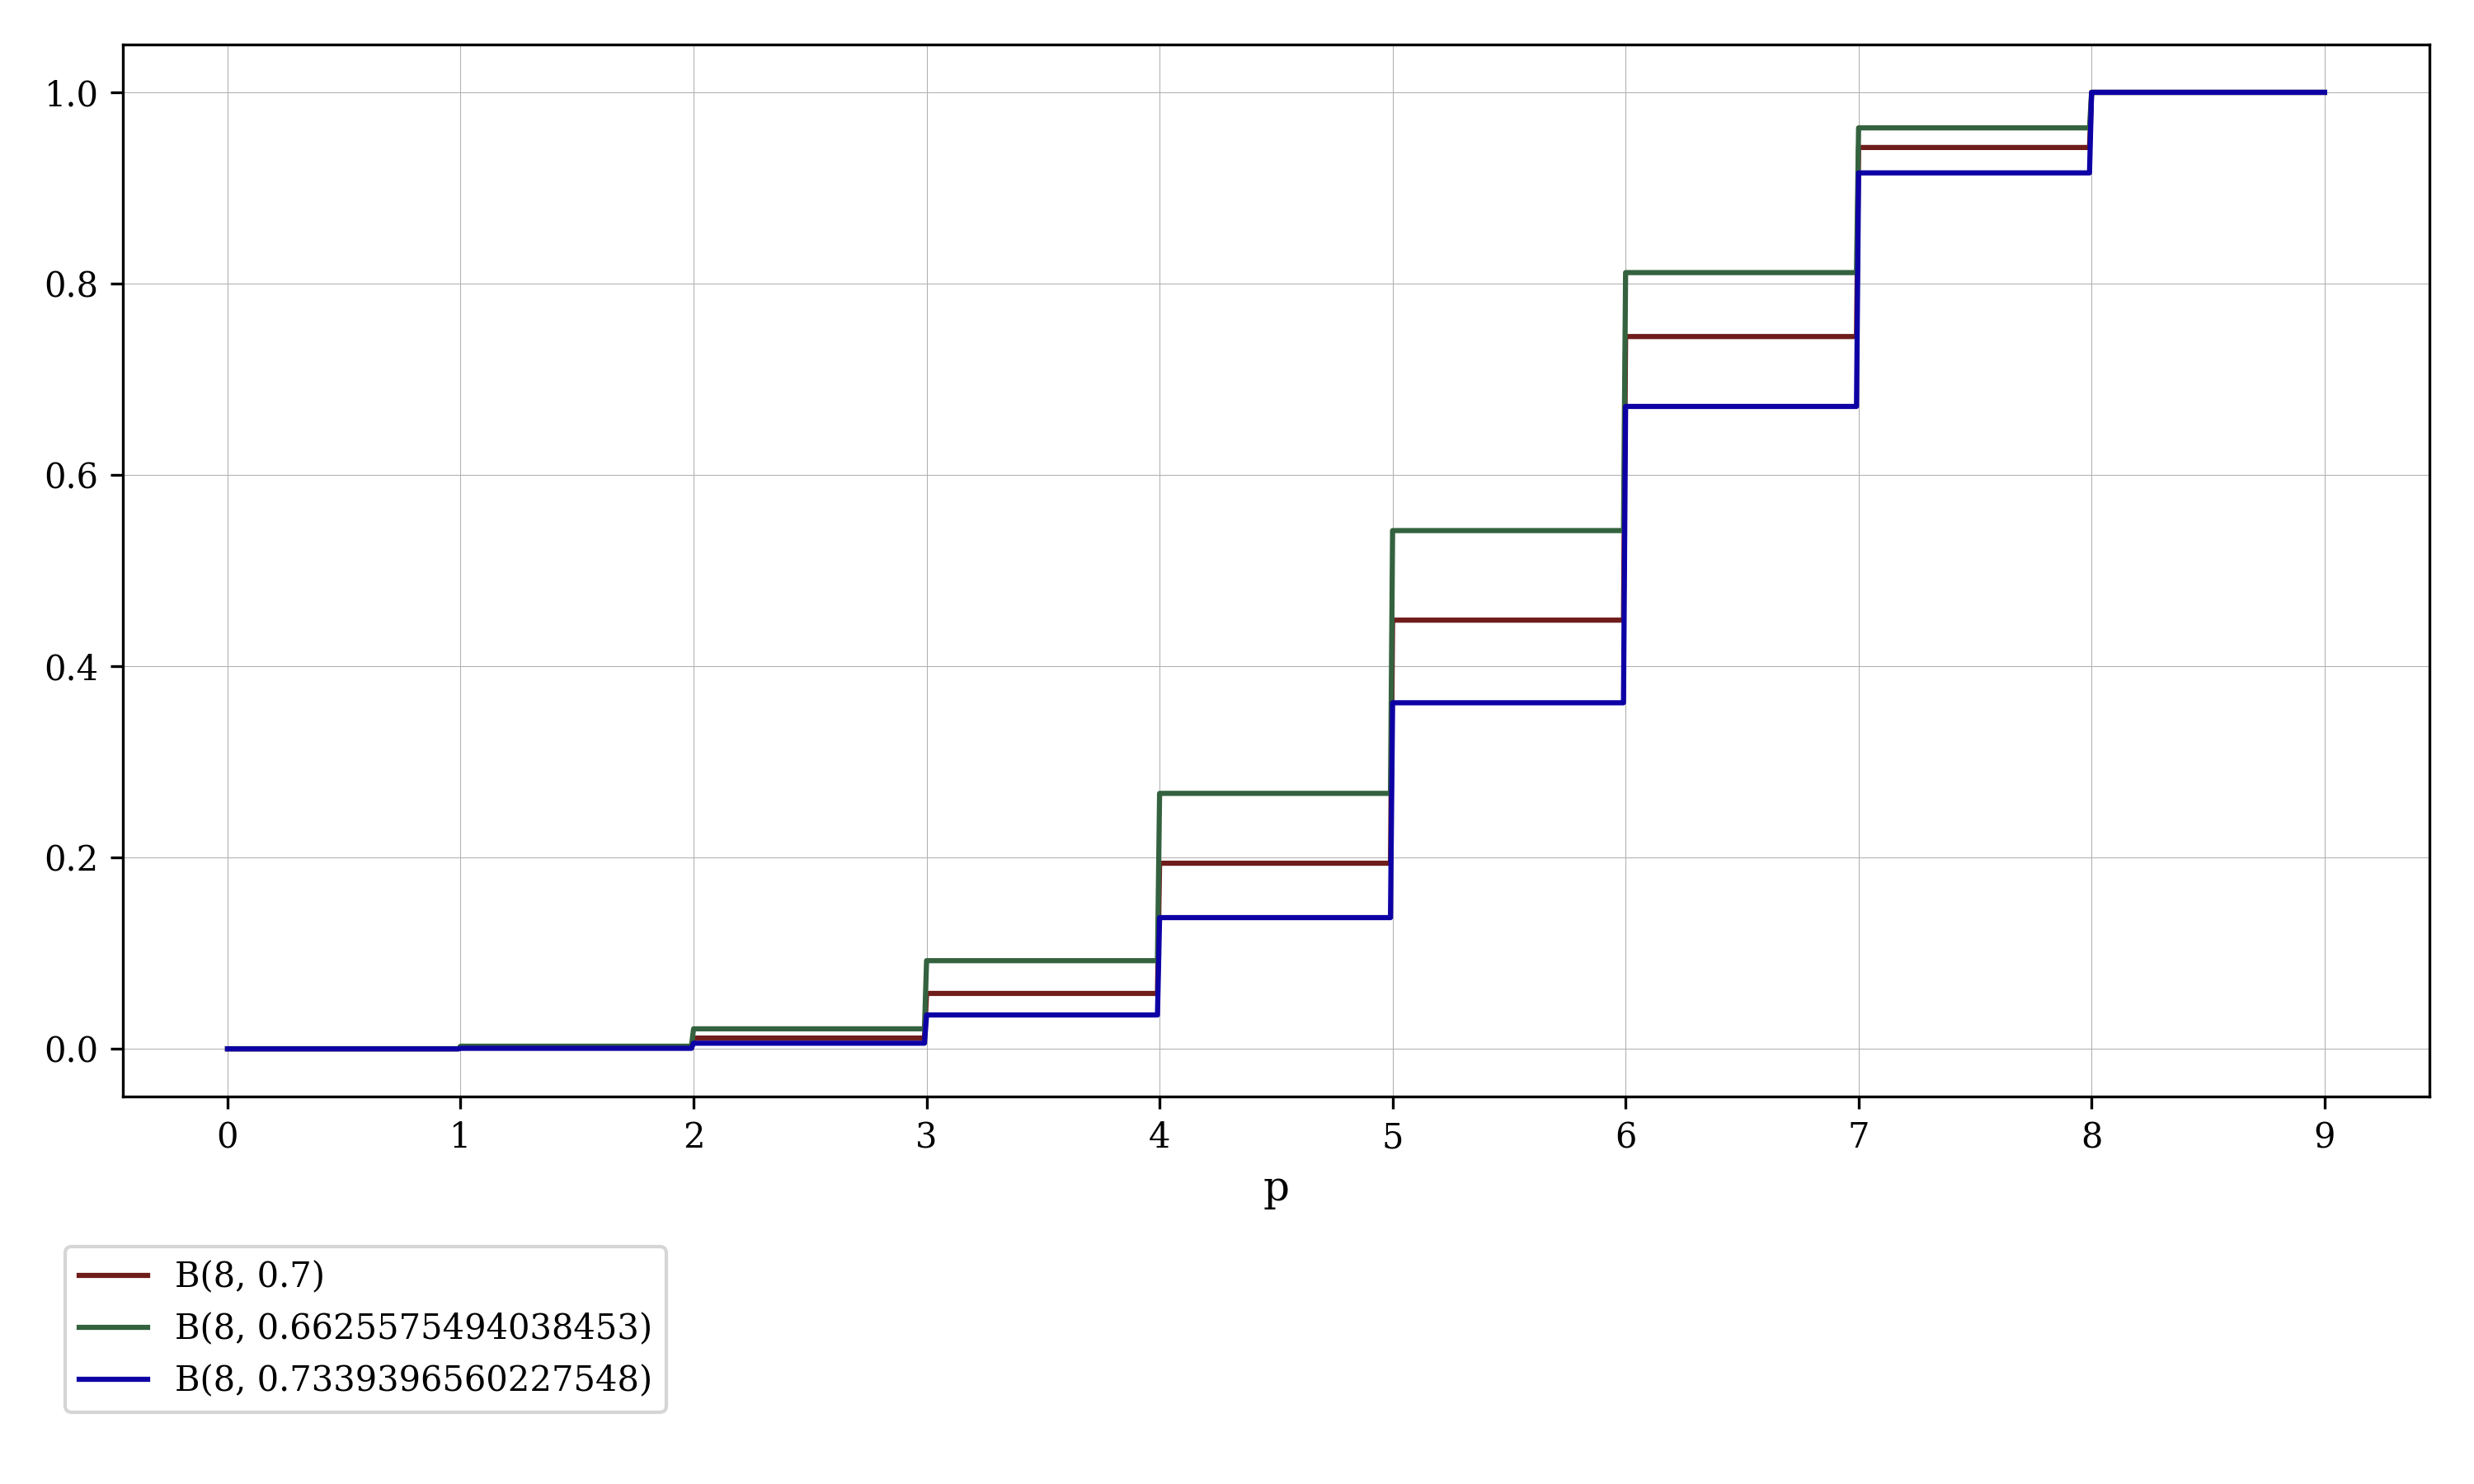
\includegraphics[width=1\textwidth]{B_step}
\end{center}

\section*{Вывод}\vspace{-20pt}\rule{\linewidth}{0.1mm}

В ходе проделанной лабораторной работы были получены доверительные интервалы для значения 
параметра $p$ биноминального распределения с помощью двух методов: по Клопперу – Пирсону и с 
использованием центральной предельной теоремы. Полученные результаты согласуются с истинным 
значением параметра $p$, границы доверительных интервалов найденные разными методами мало отличаются 
ввиду большого объема выборки, а сами доверительные интервалы становятся шире с увеличением степени 
доверия. Таким образом, показана хорошая применимость данных методов для нахождения границ доверительных 
интервалов для оценки значения неизвестного параметра распределения.

% ---------------------------------------CODE---------------------------------------

\newpage

\section*{Приложение}\vspace{-20pt}\rule{\linewidth}{0.1mm}

Программный код, с помощью которого была выполнена данная лабораторная работа.\\

\begin{center}
    \begin{lstlisting}[language=Python]
import numpy as np
import scipy as sp
import matplotlib.pyplot as plt

from IPython.display import display, Math

np.set_printoptions(suppress=True)

PRECISION = 5

k_ = 8
p_ = 0.7
n_ = 140

alpha_ = 0.01

factorial = lambda x : sp.special.factorial(x)
Cnk       = lambda n, k : \
                factorial(n) / (factorial(k) * (factorial(n - k)))
cout      = lambda name, arr : \
                print(f'{name}:\n {np.round(np.array(arr), PRECISION)}')

def decorate_plot(ax, xticks, loc=(-0.025, -0.3)):
    # Define font sizes
    SIZE_TICKS = 10

    # axis names
    ax.set_xlabel('p')

    ax.set_xticks(xticks)

    # Adjust the font size of the tick labels
    ax.tick_params(axis='both', which='major', labelsize=SIZE_TICKS)

    # plt.legend(fontsize=10, loc='lower left')
    plt.legend(fontsize=10, loc=loc)

    # Update font settings
    plt.rcParams.update({'font.family': 'serif', 'font.size': 12})

    # Adjust layout
    plt.tight_layout()

def B(k, p, n):
    q = 1 - p
    P = [Cnk(k, j) * p**j * (q)**(k - j) for j in range(k+1)]
    # cout('P', P)

    Cumulative_P = [P[i] + sum(P[:i]) for i in range(k+1)]
    # cout('cumulative P', Cumulative_P)

    Y = np.random.uniform(low=0, high=1, size=n)
    # cout('Y', Y)

    def k_alg(u, r):
        i = 0
        for j in range(len(u)):
            if r < u[j]:
                break
            i += 1
        return i
    X = [k_alg(Cumulative_P, Y[j]) for j in range(n)]
    # cout('X', X)

    return X

X = B(k_, p_, n_)
cout(f'B({k_},{p_}) of size {n_}', X)

overlineX = 1 / len(X) * sum(X)
display(Math(f'\\overline{{X}}: {overlineX}'))

K_Stat = sum(X)
display(Math(f'K(\\overrightarrow{{X}}_n): {K_Stat}'))

quantile = lambda alpha, n, p : sp.stats.binom.ppf(alpha, n, p) # n * k

def plot(filename):
    # Define colors
    RED = '#6F1D1B'
    GREEN = '#34623f'
    BLUE = '#0d00a4'

    # Create the figure and axis
    _, ax = plt.subplots(figsize=(8, 6))

    # alpha / 2
    alpha = alpha_ / 2
    x_values = np.linspace(0, 1, 100)
    y_values = [quantile(alpha, n_*k_, p) for p in x_values]
    ax.plot(x_values, 
            y_values, 
            color=BLUE, 
            linestyle='-', 
            linewidth=1.5, 
    label=f'$\\text{{quantile}}({alpha})\\text{{ for B}}({n_*k_}, \\text{{p}})$')

    # 1 - alpha / 2
    alpha = 1 - alpha_ / 2
    x_values = np.linspace(0, 1, 100)
    y_values = [quantile(alpha, n_*k_, p) for p in x_values]
    ax.plot(x_values, 
            y_values, 
            color=GREEN, 
            linestyle='-', 
            linewidth=1.5, 
    label=f'$\\text{{quantile}}({alpha})\\text{{ for B}}({n_*k_}, \\text{{p}})$')

    # Draw the horizontal line y = K_Stat
    ax.axhline(y=K_Stat, 
               color=RED, 
               linestyle='-', 
               label=f'$K(\\overrightarrow{{X}}_n): {K_Stat}$')

    # Call the decoration function
    decorate_plot(ax, np.arange(0, 1+0.1, 0.1))

    plt.grid(linestyle='-', linewidth=0.25)

    # Save the figure
    plt.savefig(f'{filename}.png', dpi=300, transparent=True)


    # Show the plot
    plt.show()

plot('quantiles')

# numerically

alphas_ = [0.1, 0.05, 0.02] + [alpha_] 

for alpha in alphas_:

    foo1 = lambda p : quantile(1 - alpha / 2, n_*k_, p) - K_Stat
    foo2 = lambda p : quantile(alpha/2, n_*k_, p) - K_Stat

    underlineP = sp.optimize.brentq(foo1, 0, 1, xtol=1e-6)
    overlineP  = sp.optimize.brentq(foo2, 0, 1, xtol=1e-6)

    print(f'{alpha}: {np.round(underlineP, PRECISION)}',end=' '*5)
    print(f'{alpha}: {np.round(overlineP, PRECISION)}')

# Klopper-Pirson

for alpha in alphas_:
    underlineP = lambda alpha : \
                    sp.stats.beta.ppf(alpha/2, 
                                      K_Stat, 
                                      n_ * k_ - K_Stat + 1)
    overlineP  = lambda alpha : \
                    sp.stats.beta.ppf(1-alpha/2, 
                                      K_Stat + 1, 
                                      n_ * k_ - K_Stat)

    print(f'{alpha}: {np.round(underlineP(alpha), PRECISION)}',end=' '*5)
    print(f'{alpha}: {np.round(overlineP(alpha), PRECISION)}')

# CPT

def find_p(alpha):
    SE = np.sqrt(overlineX * (k_ - overlineX) / (n_ * k_)) / k_

    quantile = sp.stats.norm.ppf(alpha / 2)

    lowerBound = overlineX / k_ + quantile * SE
    upperBound = overlineX / k_ - quantile * SE

    return (lowerBound, upperBound)

for alpha in alphas_:
    underlineP, overlineP = find_p(alpha)
    print(f'{alpha}: {np.round(underlineP, PRECISION)}',end=' '*5)
    print(f'{alpha}: {np.round(overlineP, PRECISION)}')

def plot(filename):
    # Define colors
    RED = '#6F1D1B'
    GREEN = '#34623f'
    BLUE = '#0d00a4'

    # Create the figure and axis
    _, ax = plt.subplots(figsize=(10, 6))

    underlineP = lambda alpha : \
                    sp.stats.beta.ppf(alpha/2,   
                                      K_Stat,     
                                      n_ * k_ - K_Stat + 1)
    overlineP  = lambda alpha : \
                    sp.stats.beta.ppf(1-alpha/2, 
                                      K_Stat + 1, 
                                      n_ * k_ - K_Stat)

    x_values = np.linspace(0, k_+1, 1000)
    
    # B(k, p)
    y_values = sp.stats.binom.cdf(x_values, k_, p_)
    ax.plot(x_values, 
            y_values, 
            color=RED, 
            linestyle='-', 
            linewidth=1.5, 
            label=f'B({k_}, {p_})')
    
    # B(k, underline p)
    p = underlineP(alpha_)
    y_values = sp.stats.binom.cdf(x_values, k_, p)
    ax.plot(x_values, 
            y_values, 
            color=GREEN, 
            linestyle='-', 
            linewidth=1.5, 
            label=f'B({k_}, {p})')

    # B(k, overline p)
    p = overlineP(alpha_)
    y_values = sp.stats.binom.cdf(x_values, k_, p)
    ax.plot(x_values, 
            y_values, 
            color=BLUE, 
            linestyle='-', 
            linewidth=1.5, 
            label=f'B({k_}, {p})')

    # Call the decoration function
    decorate_plot(ax, np.linspace(0, k_+1, 10))

    plt.grid(linestyle='-', linewidth=0.25)

    # Save the figure
    plt.savefig(f'{filename}.png', dpi=300, transparent=True)

    # Show the plot
    plt.show()

plot('B_step')
    \end{lstlisting}
\end{center}

\end{document}
